% Reader-facing manuscript. Frozen scientific outputs are not re-estimated.
\documentclass[11pt]{article}
\usepackage[margin=1in]{geometry}
\usepackage{amsmath,amssymb,booktabs,array,longtable,graphicx,xurl}
\usepackage[hidelinks]{hyperref}
\usepackage{tikz,placeins,needspace}
\usetikzlibrary{arrows.meta}
\setlength{\emergencystretch}{3em}
\newcommand{\R}{\mathbb{R}}
\newcommand{\ES}{\operatorname{ES}}
\newcommand{\supp}[1]{\href{supplement.pdf\##1}{scientific supplement}}
\newcommand{\audit}[1]{\href{audit-notes.pdf\##1}{audit record}}
% Generated from original public aggregate values; no inference.
\newcommand{\FullES}{477.85}
\newcommand{\InertialES}{824.73}
\newcommand{\FullFDE}{1326.09}
\newcommand{\FullADE}{636.11}
\newcommand{\InertialDelta}{-346.87}
\newcommand{\PointRowFull}{Full & 73.77 & 332.31 & 812.26 & 1326.09\\}
\newcommand{\PointRowGMM}{GMM & 71.92 & 323.79 & 792.99 & 1299.11\\}
\newcommand{\PointRowdtThreeHundred}{dt300 & 75.88 & 340.10 & 825.76 & 1335.73\\}
\newcommand{\PointRowInertial}{Inertial & 31.17 & 237.93 & 934.03 & 2095.78\\}

\author{}
\date{Public review revision, 9 October 2026; authorship unconfirmed}

\title{Horizon-dependent Performance and Undercoverage in\\Probabilistic Movement Forecasting}
\begin{document}
\maketitle
\begin{abstract}
We study the relation between distributional score, position accuracy and
uncertainty coverage for fitted stochastic movement predictors. Evaluation
uses 46 unique recording-hash blocks selected retrospectively for temporal
and future-route map support, five fixed simulation seeds and 512 particles.
Horizons are nominal 1, 5, 15 and 30 minutes in the saved clock; physical clock
provenance and participant independence are not established, and this is not
a previously untouched evaluation cohort. Full's equally weighted energy
score (ES) is \FullES\ m, versus \InertialES\ m for deterministic constant-speed
extrapolation. The inertial reference is better at 1 and 5 minutes and Full
at 15 and 30 minutes. Full's nominal 90\% marginal prediction disk covers
only 46.52\% of 30-minute targets. The original 21 primary-method comparisons
yield 14 practically equivalent and seven inconclusive finite-algorithm
states; none establishes an effect wholly beyond the registered practical
margin. Resolution-invariant states remain inconclusive. Terrain-family
inference is unavailable because required forecasts failed; this does not
establish that terrain is ineffective. These conditional findings motivate
joint reporting of score, point error, coverage and evidence availability,
not an operational reliability claim or general ranking of algorithms.
\end{abstract}

\noindent\textit{Evidence version.} The once-only saved-output audit and the
fixed-budget public aggregate replay are complete. This revision reorganizes
their results without changing forecasts, fits or statistical rules. The
\supp{sec:models} supplies full scientific specifications and tables; the
\audit{sec:audited-review-update} supplies version, execution and review
history. Authorship, route-publication permission and human acceptance remain
separate decisions.

\section{Introduction and research scope}\label{sec:introduction}\hypertarget{sec:introduction}{}
A useful movement forecast must describe plausible future positions without
hiding uncertainty. A low distributional score, a small position error and a
well-calibrated prediction region answer different questions. They need not
improve together. We examine these distinctions in a limited collection of
interpretable fitted stochastic predictors, rather than proposing a new
general stochastic differential equation (SDE) theory.

Continuous-time correlated random walks model irregularly observed movement
and persistence~\cite{johnson2008}. Switching state-space models represent
latent regimes~\cite{ghahramani2000}; their regime identities require care
when parameters are transferred between batches. Step-selection models link
movement and environmental selection~\cite{avgar2016,avgar2017correction},
but that relation cannot be inferred from arbitrary unbalanced feature
ablations. Learned trajectory models~\cite{gupta2018,salzmann2020} and neural
SDE path generators~\cite{kidger2021} provide broader context, not executed
performance baselines for this study. Interpretable stochastic system
identification~\cite{gao2024} motivates explicit drift and noise specifications.
Our contribution is a bounded empirical examination of horizon-specific
trade-offs and undercoverage in the predictors actually evaluated.

Proper distributional scoring~\cite{gneiting2007,gneiting2008} rewards a
predictive distribution relative to realized targets, but does not certify
that a particular marginal region attains its nominal coverage. Consequently
we keep ES, error of the ensemble mean, and disk coverage/size separate.
The simple inertial reference establishes the short-versus-long-horizon
reversal; internal comparisons then identify which implemented procedures
change these diagnostics. They do not establish the necessity of a complex
random model relative to a simple probabilistic motion baseline.

The original registered questions remain traceable: RQ1 asks about method
component comparisons; RQ2 asks about terrain increments beyond the history
baseline. RQ1 now has conditional fixed-algorithm results, with several
comparisons changing multiple factors or sharing parameters. RQ2 has a
design and an explicit unavailable result, not a positive or null terrain
answer. The paper is organized around what this evidence can actually show.

\section{Predictors and what the comparisons change}\label{sec:models}\hypertarget{sec:models}{}
\subsection{Ordinary Full and its actual inputs}
Let $X=(X_e,X_n)^\top$ denote position in the saved local coordinate frame
(metres), and $t$ the saved time coordinate (seconds). The origin is the last
permitted prefix position. The first visible position anchors the frame.
Full uses three fitted modes and the position dynamics
\begin{equation}\label{eq:ordinary-full}
 dX_t=\Theta_{m_t}^{\top}\psi(X_t,t)\,dt+L_{m_t}\,dW_t,
 \quad \psi=(1,X_e,X_n,S)^{\top},\quad L_mL_m^{\top}=Q_m=\tau R_m.
\end{equation}
Here $\Theta_m$ gives drift in m/s, $S$ is the solar/calendar input computed
from the retained absolute tick, and $R_m$ is a fitted rate-residual covariance
in m$^2$/s$^2$. Its conversion to $Q_m$ uses the model observation interval
$\tau$, not the integration step $h$. The physical interpretation of seconds
and daylight remains conditional on clock provenance (Section~\ref{sec:data}).
Saved mixing weights $\pi_m$ come from fitting/adaptation, not a posterior
update from a new visible prefix.

\begin{table}[htbp]\centering
\caption{Actual prefix information. A buffer being updated is not proof that
the drift reads it. The three routes are not interchangeable.}\label{tab:inputs}
\begin{tabular}{p{.19\linewidth}p{.73\linewidth}}\toprule
Route & Drift inputs and interpretation\\\midrule
Ordinary Full & Position, calendar proxy and saved $\pi$; no initial speed
or signed recent heading at fixed frame, position, clock and random stream.\\
Explicit features & Speed norm and position-radial direction; also changes
three modes to one. Radial direction is not velocity direction.\\
Terrain base/full & Secant velocity and signed three-position history,
with retained map features in all-terrain.\\\bottomrule
\end{tabular}\end{table}
Changing a prefix can change the frame anchor, the numerical position and
origin-specific random-stream identity. Full therefore does not ``ignore
the prefix''. However, after these inputs are held fixed, changing only
initial velocity leaves ordinary Full unchanged. On the explicit route,
reversing velocity at the same norm does not change its speed feature;
the position-radial direction has its own zero-position convention.

Each training/adaptation/validation batch is independently sorted by segment
net-displacement heading and split into three rank groups. Mode labels
0/1/2 in code correspond to mathematical modes 1/2/3. Training has
110/109/109 segments, adaptation 26/25/25, and validation 27/27/27; these
are segment counts, not transition frequencies or $\pi_m$. Reptile tasks
sort their own batches. Blending uses matching indices without a semantic
matching step. Missing per-mode direction support and intermediate parameter
snapshots prevent a claim that these indices represent matched behaviours.
Thus transfer results concern this sorting-and-interpolation procedure,
not meta-learning or adaptation in general. Full tie/branch-cut rules and
the original 84 groups, 30 eligible tasks and 258 task segments are retained
in the \supp{sec:reptile-task-accounting}.

\subsection{Fitting, calibration and propagation}
Base drift fitting uses ridge regression on displacement rates. Ordinary
residual covariance is centred with denominator $n_m-1$ and a $10^{-8}I$
jitter before the saved scale and $Q=\tau R$ conversion. Full calibrates a
finite scale grid while fixing drift-blend coefficient $\eta=0$.
Mixed/pure-ES additionally fit validation drift and choose $\eta,s$ on a
finite grid, whose largest drift blend is $0.5$. These are calibration
programs, not end-to-end ES training or global optima.

The selection proxy uses one-step rate residuals and a single Gaussian with
the unweighted arithmetic covariance $M^{-1}\sum_mR_m$, not the $\pi$-weighted
multi-mode, multi-step position distribution eventually scored. GMM first
fits a pooled drift, groups its residuals once by
$\arg\max(r_e,r_n,-r_e-r_n)$, then refits group-specific drifts. Validation
residuals instead select components using segment-heading mode labels.
This is a real label mismatch, not a likelihood-EM fit. The proxy/task
mismatch is a plausible explanation for undercoverage, but the current
results do not identify it as the cause.

The registered integration cap is $h=5$ saved seconds, with $N=512$
particles and five fixed seeds. FP denotes conditional Gaussian moment
propagation evaluating nonlinear conditions at the conditional mean; MC
evaluates them along individual paths. Local affine substeps may be exact,
but this is not an exact solution of a globally nonlinear SDE or global
Fokker--Planck equation~\cite{kloeden1992}. The four targets are generated
from a continuing joint stochastic path, not four independently sampled
marginals. Common random indices require the same grid, origin, pair and
seed; they neither prove variance reduction nor Brownian consistency across
different step grids. All original propagation and numerical-qualification
limits are retained in the \supp{sec:method-model}.

\begin{table}[htbp]\centering
\caption{Scientific interpretation of registered procedure comparisons.
The original five families, 28 identities and 21 primary contrasts are kept;
identities are not counts of independent algorithms.}\label{tab:actual-changes}
\begin{tabular}{p{.23\linewidth}p{.69\linewidth}}\toprule
Comparison & What changes; what must not be attributed\\\midrule
Pointwise / single / explicit & Mixing or representation; explicit also
changes mode count. Not an isolated velocity-feature effect.\\
QMLE vs Full & Saved $\Theta,R,\pi$ are identical. Finite random score
differences do not show a training-objective effect.\\
Mixed vs pure-ES & Same saved parameters; both add validation drift fitting
relative to Full. Not an isolated loss-function comparison.\\
Scratch / Reptile / drift-only & Implemented fit/blend procedures. Mode
indices are not proven semantically aligned; two-step is not a new sequential
optimizer~\cite{nichol2018}.\\
Observation interval & Fit data, noise binding $Q=\tau R$ and history/mode
cadence change together; maximum integration $h$ remains 5 s.\\
EM / Euler / d2 & EM and Euler are update aliases. Two d2 score routes share
predictions and common scoring; they do not independently validate their
native estimators.\\
MC / CRN & Propagation procedures with their named Full20 control, not
generic comparisons against an interchangeable pooled Full.\\\bottomrule
\end{tabular}\end{table}
Parameter equality, array equality, score equality and random-stream equality
are distinct claims. Full01/07/11/18/20 and the additional Full reference
remain separately named; their saved scores are never pooled to make an
artificial common control.

\subsection{Terrain branch and history feedback}
Terrain base is not ordinary Full. It fits a shared history drift $B_0$
then independently fits a residual conditioner and diffusion for each of
ten terrain configurations:
\begin{equation}\label{eq:terrain-summary}
 dX_t=\{B_0\phi_{\rm hist}(t)+C_g\tilde f_g(X_t,t)\}\,dt+L_g\,dW_t,
 \qquad L_gL_g^{\top}=Q_g.
\end{equation}
There are 404 training and 81 validation transitions, using each window's
first future transition with equal row weight. The first ridge minimizes
an unnormalised squared sum with $\rho=10^{-6}$; the correction minimizes
mean loss with $\lambda=10^{-4}$ (normal-equation penalty $404\lambda=0.0404$).
Neither is joint optimisation. Terrain $Q_g=n^{-1}\sum_i\Delta t_i\zeta_i\zeta_i^\top$
is an uncentred rate-residual second moment, without a degrees-of-freedom
correction, and is not the ordinary method's $R_m$.

\begin{figure}[htbp]\centering
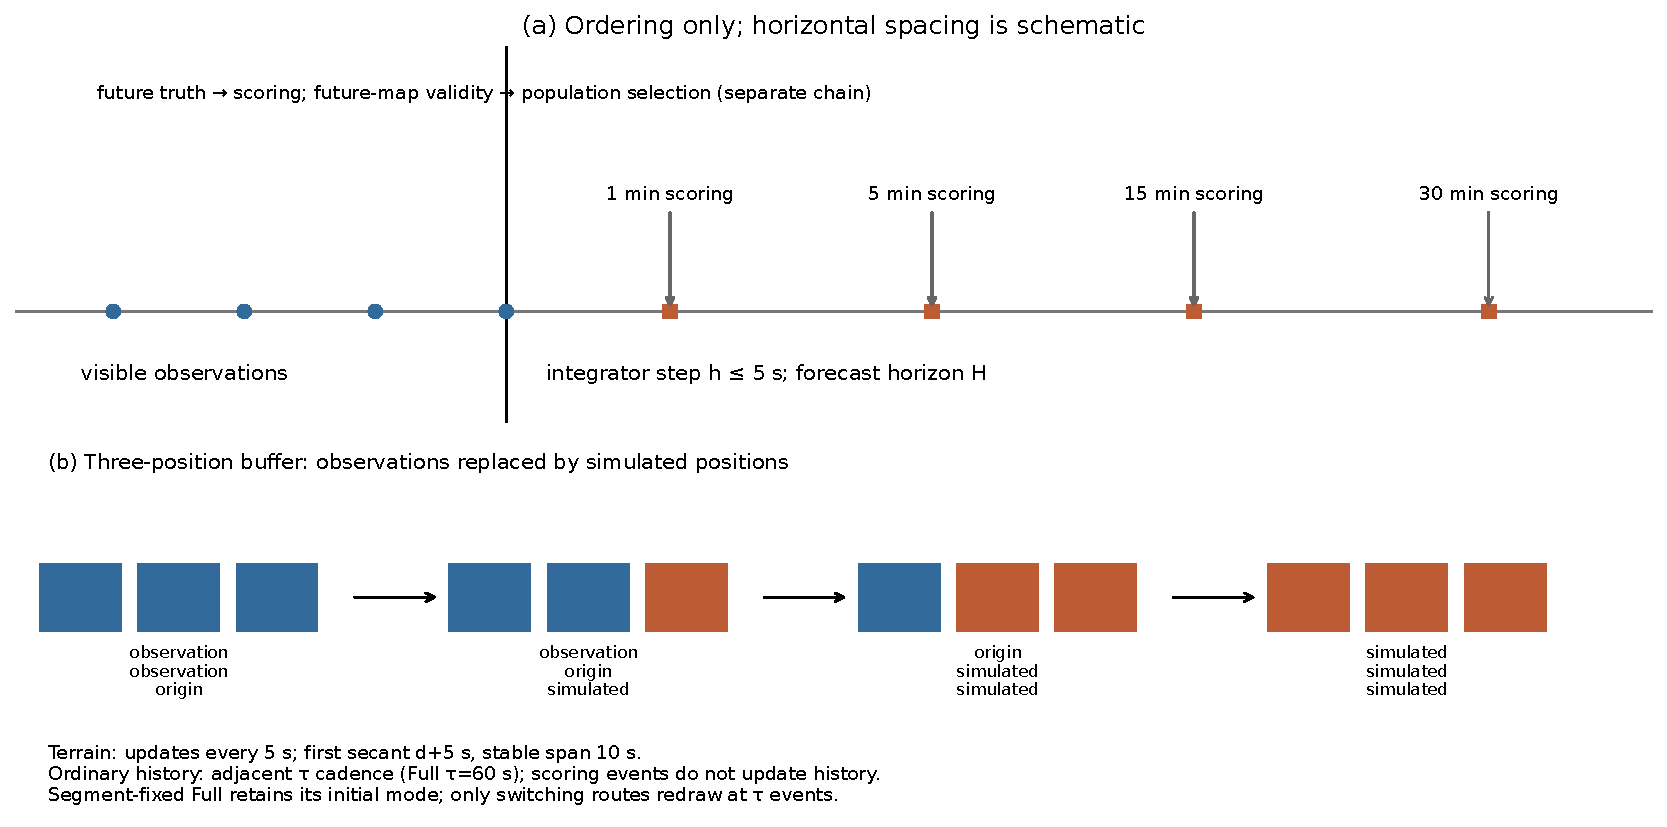
\includegraphics[width=\linewidth]{../figures/revision46-v1/revision46-history-timeline.pdf}
\caption{Observed prefix and simulated history. $\tau$ is the observation/model
cadence, $h$ the integration step and $H$ the forecast horizon. Terrain updates
its three-position buffer on 5 s events; once entirely simulated, its secant
spans 10 s. Ordinary Full has a separate $\tau=60$ s cadence. Future observations
enter scoring only; scoring an event does not itself update history.}
\label{fig:history-timeline}\end{figure}

The feature groups are history, retained-road subset, river, cover and surface,
including road--cover and surface--history interactions. Road/river direction
points towards the nearest feature point, not along its tangent or flow.
The road filter excludes bridleway, cycleway, footway, path, pedestrian,
steps and track; it is not the complete pedestrian network. Surface features
separate the signed history, uphill and contour directions; slope does not
multiply their directional dot products. Geometry and the ten-configuration
matrix are in the \supp{fig:terrain-geometry}.

Training/validation selected masks are all one, while future simulated
queries can be invalid. The code zero-fills invalid numerical features and
adds masks; robustness to such out-of-training-distribution inputs has not
been learned or demonstrated. With penalised intercept and $K$ constant-one
masks, the minimum constant-subspace penalty is
\begin{equation}\label{eq:constant-penalty}
 \min_{\sum_{j=0}^{K}a_j=c}\frac{\lambda}{2}\sum_{j=0}^{K}a_j^2
 =\frac{\lambda c^2}{2(K+1)}.
\end{equation}
Base has $K=2$ and all-terrain $K=28$, so this denominator changes from
3 to 29. This is not a 9.7-fold change of the entire model's penalty.
Unstandardised scales, redundant columns, independent refitting and diffusion
changes further confound pure information attribution. Even complete forecasts
would establish configuration increments, not isolated terrain effects.

\section{Data, targets and evaluation}\label{sec:data}\hypertarget{sec:protocol}{}
\subsection{A retrospectively selected population}
The released data contain 12,370 windows from 1,094 recording-hash blocks.
Temporal eligibility leaves 127 windows/89 blocks; joint feature validity
leaves 106/73; the fixed primary-origin selection leaves 46/46.
The 130 windows having at least 1,800 s follow-up are not identical to the
127 passing all temporal criteria. Among temporally eligible windows, 21
fail joint map support. The 27 eligible but unselected blocks and extra
windows are selection outcomes, not forecast failures.

\begin{figure}[htbp]\centering
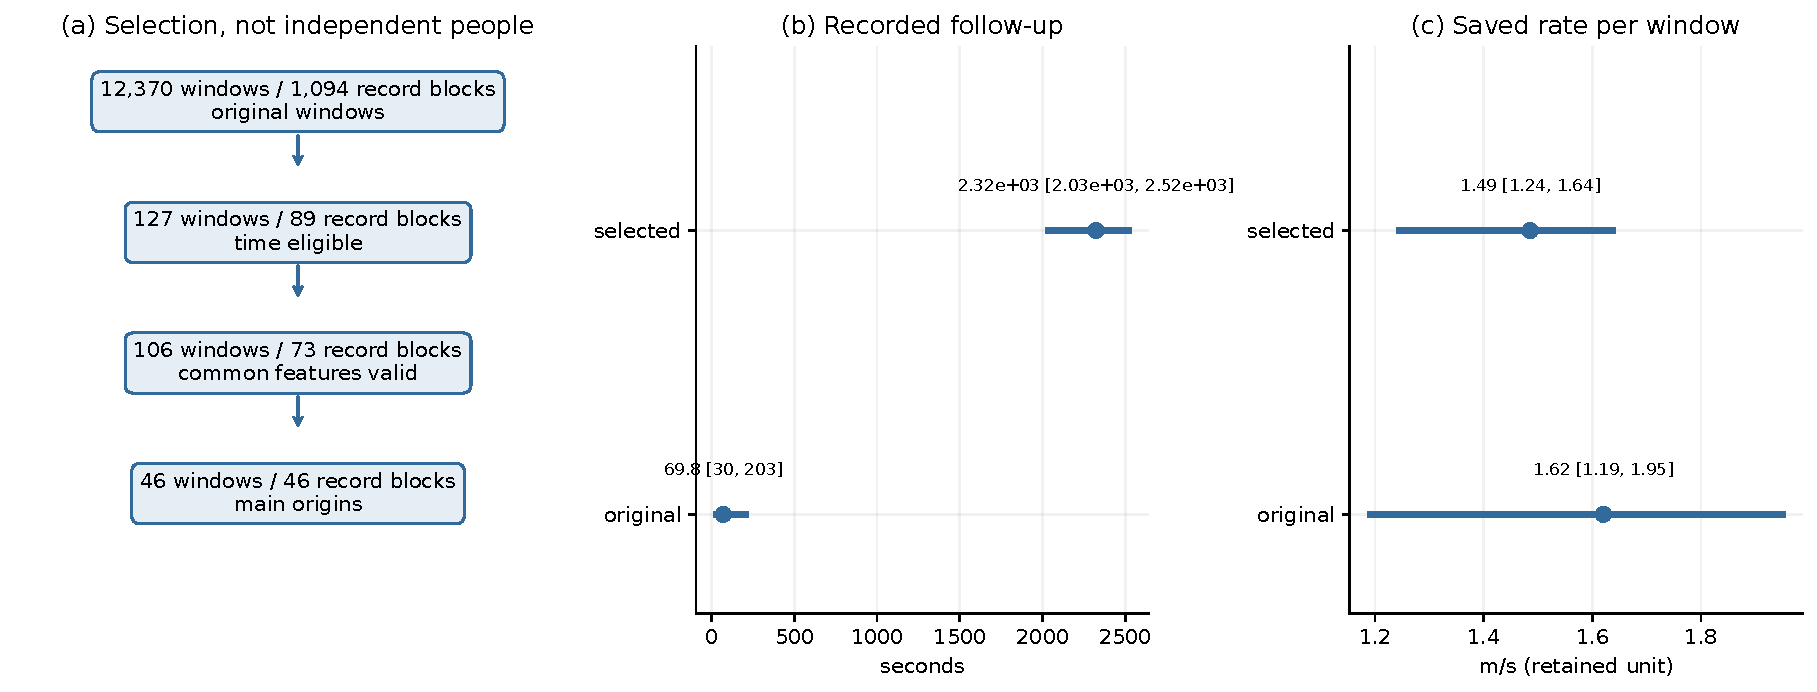
\includegraphics[width=\linewidth]{../figures/revision46-v1/revision46-population.pdf}
\caption{Window and recording-block funnel, with released versus selected
follow-up duration and saved speed median/IQR. These are population
descriptions, not predictor estimates. Eligibility tests map validity along
the observed future route; it cannot be determined at deployment from the
prefix alone.}\label{fig:population}\end{figure}

Future true positions are not inputs to prediction: online queries use
simulated positions. Nevertheless, future-route support is used to select
this evaluation population, an important post-hoc restriction. The selected
cohort spans 12 countries and 27 source labels; 33/46 blocks are from Great
Britain, Belgium or Luxembourg. It is neither a globally representative
sample nor a deployment-qualified cohort. The evaluation data were used
previously; the complete influence of earlier inspection on design choices
is not recoverable. It is not a fresh blinded holdout.

Exact saved-identity and full-sequence checks do not identify participants,
nearby routes, repeated visits or formatting-modified duplicates. The block
resampling therefore depends on unverified independence/exchangeability
assumptions. Six known-velocity and six point-only cases reuse the primary
records: there are 46 unique recording blocks and 58 origin--mode cases,
not 58 participants or independent blocks.

\subsection{Saved-clock horizons and metric definitions}
Forecasts stop at the actual matched target, rather than interpolating an
observation to an exact nominal horizon. Nominal 1/5/15/30 minute targets
have retained elapsed-time ranges 49--67/294--305/889--910/1785--1814 s.
Relative time reconstructed in the R1 data procedure and the condition tick
used in prediction are separate objects. Exact tick joins and datetime
precision do not authenticate physical acquisition time or UTC. An absolute
offset affects solar/calendar interpretation; a relative-scale distortion
affects rates, diffusion units and the meaning of a physical 30 minutes.
No timezone correction is guessed. Results throughout are for the saved
clock's nominal horizons; $S$ is a calendar proxy, not a validated daylight
mechanism. Source reconciliation is in the \audit{sec:source-reconciliation-details}.

For particles $x_1,\ldots,x_N$ and target $y$ at a matched time, the original
finite-ensemble score is
\begin{equation}\label{eq:finite-es}
 \ES_N=\frac1N\sum_i\|x_i-y\|
       -\frac1{2N^2}\sum_{i,j}\|x_i-x_j\|.
\end{equation}
The $N^2$ denominator and diagonal convention are preserved, not silently
replaced by $N(N-1)$. ES has units of metres; lower is better. Weighted ES
is the equally weighted average over the four targets. Mean-position error
is $e_j=\|\bar x_j-y_j\|$, with
$\mathrm{ADE}=\tfrac14\sum_{j=1}^4 e_j$ and $\mathrm{FDE}=e_4$.
ADE is not a dense-path integral; FDE is neither best-particle error nor
mean particle error. Marginal particle-centred quantile disks are evaluated
for coverage and area at each horizon, not as joint path regions. Average
area is $\mathrm{E}[\pi r^2]$, not $\pi\mathrm{E}[r]^2$.

The completed inventory is $28\times58\times5=8120$ method forecasts,
$10\times58\times5=2900$ terrain forecasts, 290 same-grid replay forecasts
and 58 inertial paths: 11,368 score slots. The registered scientific 11,020
contain 11,015 successes and five failures; all score slots contain 11,363
successes and those same five failures. A score-slot count is not an array
audit scope or number of independent observations.

\subsection{Conditional paired inference}
Within each recording block, the five fixed seeds are averaged before paired
block inference. They quantify simulation variation, not independent people
or training uncertainty. Original family-wise simultaneous bootstrap-$t$
intervals use 2,000 draws per stream and shared within-family block indices;
Holm-adjusted zero tests~\cite{holm1979} have a separate role. The practical
margin is $\delta=41.100259$ m, 5\% of validation inertial ES, not a validated
search-and-rescue utility threshold. Planning used only three development
blocks. A five-contrast family's single tail has about ten expected draws
at probability 0.005; a four-contrast family's tail has about 12.5. These
are finite precision limitations, not a simultaneous coverage theorem
\cite{davison1997}.

All deltas are candidate minus named control; negative ES is favourable.
An interval crossing zero is not evidence of equivalence. Practical benefit
or harm requires the entire original interval beyond $-\delta$ or $+\delta$
and its original statistical, seed and qualification gates. Equivalence,
inconclusive information, unavailable evidence and failed program
qualification are different states. Zero-SD d2 aliases do not independently
demonstrate power; the dt600 comparison has low planning power. Full
procedure and precise endpoints remain in the \supp{sec:bootstrap-table-detail}.

\section{Results}\label{sec:method-results}\hypertarget{sec:method-results}{}
\subsection{Simple extrapolation first: the horizon reversal}
On the same 46 primary blocks and original targets, saved weighted ES is
\FullES\ m for Full and \InertialES\ m for inertia. Their stored difference
rounds to \InertialDelta\ m, computed from unrounded values, not subtraction
of displayed means. Inertia is better at 1 and 5 minutes; Full is better
at 15 and 30 minutes (Figure~\ref{fig:inertial}). The four isolated target
times do not locate an exact crossover time. This descriptive reference
comparison is not a newly registered superiority test.

\begin{figure}[htbp]\centering
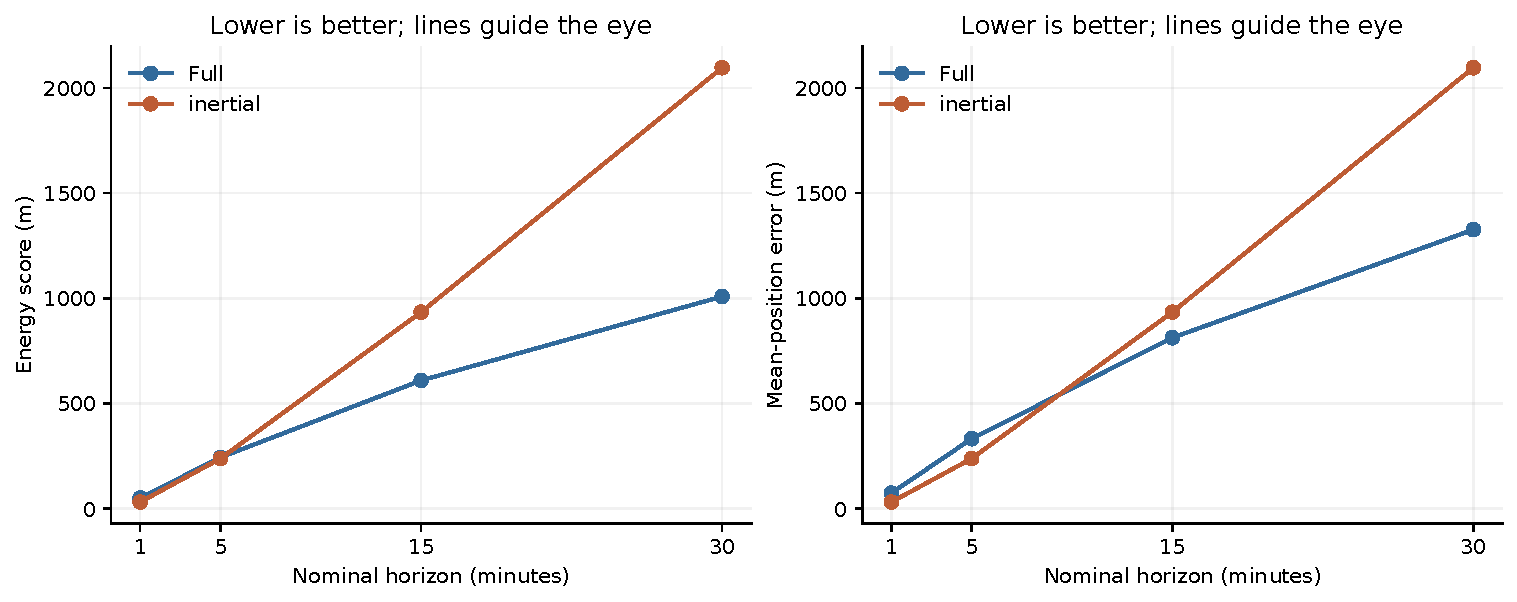
\includegraphics[width=\linewidth]{../figures/revision46-v1/revision46-inertial-horizons.pdf}
\caption{Full versus deterministic inertia at four nominal horizons.
Left: ES; right: error of the predictive mean. The curves use the original
equal-block/equal-seed summaries. Lines guide the eye, not interpolation
or evidence for a precise crossover.}\label{fig:inertial}\end{figure}

\begin{table}[htbp]\centering
\caption{Saved error of the predictive mean (m), with original target matches
and four-model scope. These are not ES or mean particle errors.}\label{tab:point-errors}
\begin{tabular}{lrrrr}\toprule
Model & 1 min & 5 min & 15 min & 30 min\\\midrule
\PointRowFull
\PointRowGMM
\PointRowdtThreeHundred
\PointRowInertial
\bottomrule\end{tabular}\end{table}
The deterministic reference is a valid point-mass distribution for ES, but
does not test whether this stochastic model is necessary. A matched
probabilistic constant-velocity state-space baseline is a separate future
experiment, not a result presented here.

\subsection{Long-horizon marginal disks are undercovered}
Full's nominal 90\% coverage is 95.65\%, 37.83\%, 35.22\% and 46.52\% at
the four targets. At one minute, the 50\% disk covers 33.04\% while the
90\% disk covers 95.65\%; at thirty minutes even the 95\% disk covers only
52.17\%. Thus a single demonstrated radius rescaling is not the explanation.
Across all 28 identities, thirty-minute 90\% coverage is 21.74--79.13\%.
The full ES/area/coverage-deviation overview is in the
\supp{fig:method-overview}; its diverging colour scale is centred on nominal
coverage, so overcoverage is not visually rewarded as ``better''.

Full's thirty-minute mean 90\% disk area is 4.534 km$^2$ and mean radius
1183.6 m; median block area is a different 4.022 km$^2$ summary.
The 300 s interval procedure has 9.109 km$^2$ mean area and 64.35\% coverage,
with FDE 1335.73 m; the 600 s procedure has 12.609 km$^2$, 79.13\% and
1340.94 m. Larger regions cover more but do not make the ensemble mean
more accurate or establish conditional calibration. No radius is retuned
after inspecting this evaluation.

\subsection{Component comparisons and conflicting metrics}
None of the 21 original simultaneous intervals lies wholly beyond the
registered $\pm\delta$ practical boundaries. The audited finite-algorithm
states are 14 practically equivalent and seven inconclusive; all
resolution-invariant states remain inconclusive. Human acceptance is not
implied. The pointwise mixture raises ES by 32.95 m relative to Full01;
the GMM difference is $-2.83$ m with an interval spanning zero. At 5 and
15 minutes GMM's descriptive ES advantage reverses at 30 minutes.

\begin{figure}[htbp]\centering
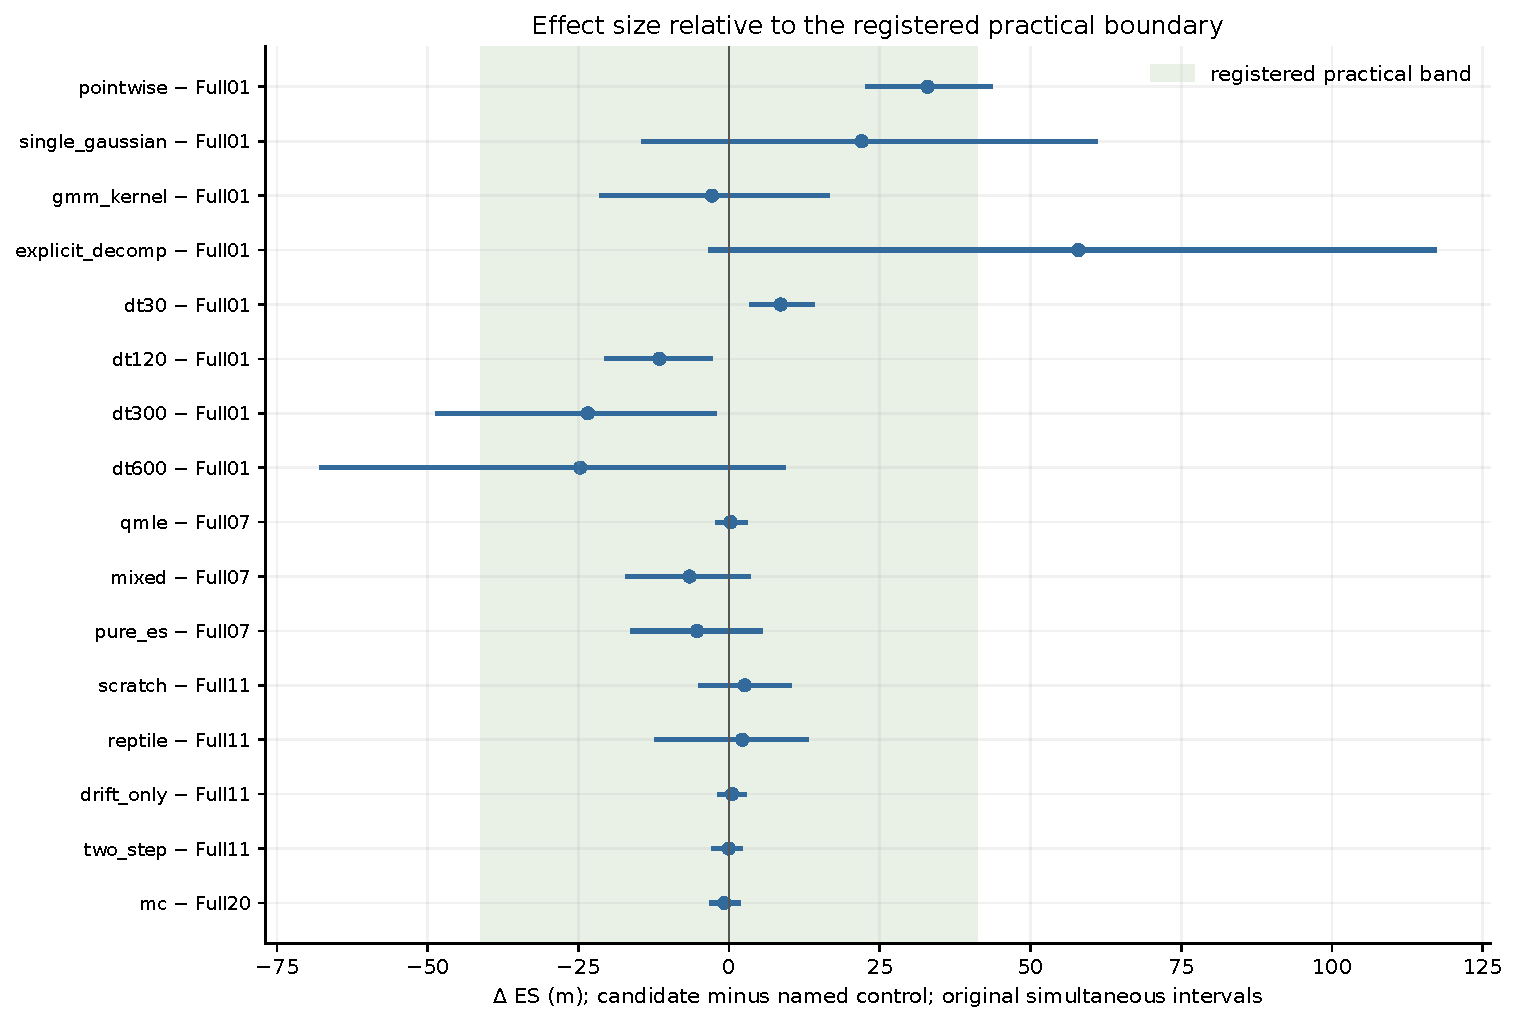
\includegraphics[width=\linewidth]{../figures/revision46-v1/revision46-practical-effects.pdf}
\caption{Original paired ES effects and simultaneous intervals, preserving
each named candidate/control and the $\pm41.10$ m practical band. Tiny
implementation-consistency contrasts are separately displayed at their own
scale in the supplement; they are not discarded or treated as scientifically
large effects. Qualification and interval location are distinct.}
\label{fig:practical-effects}\end{figure}

An ES improvement can accompany a larger endpoint error. The supplement's
family-faceted $\Delta$ES--$\Delta$FDE quadrants retain the separate Full
controls rather than joining two unrelated rankings. Seed/block plots
also distinguish two uncertainty sources: single-Gaussian seed deltas are
all positive but its block interval is $[-14.19,60.81]$ m; GMM's five are
negative but its interval is $[-21.22,16.33]$ m; dt600's five are negative
with $[-67.65,9.08]$ m. Seed-direction agreement does not settle population
uncertainty. Full five-seed tables, CRPS, endpoint particle-error quantiles
and all 120 original metric views remain available in the supplement.

\subsection{Terrain evidence and failure-dependent availability}\label{sec:terrain-results}\hypertarget{sec:terrain-results}{}
The five retained failures have different family consequences. F01
(known-velocity dt30) invalidates that mode's observation-interval family;
F02 (known-velocity single Gaussian) its model-structure family. F04
(primary all-terrain) invalidates the entire overall/LOO terrain family;
F03/F05 (primary LIO-river/LIO-road) invalidate the entire LIO family.
The overall/LOO grid has 1379/1380 successes and one failure; LIO has
1148/1150 and two failures, with no missing pending slots. These grids
share baselines and must not be added as distinct forecasts.

The original complete-family rule does not permit a successful-subset
factor ranking. ``Unavailable'' is not ``no benefit'', ``zero effect'' or
``equivalent''. Completed auxiliary tasks do not remove a retained failure.
Five primary method families are complete but still have their own
qualification states. The \supp{fig:availability} distinguishes family/mode
availability; the \audit{sec:terminal-failures} retains each failure identity
and known logging limits. Missing exception stacks preclude a causal
assertion of divergence, timeout, out-of-memory or a physical power loss.

\subsection{Development diagnostics and computational cost}
All-terrain's improved training fit with slightly worse validation fit is a
development diagnostic, not a prediction benefit. The supplement plots all
ten fit MSEs beside raw design columns/rank, separating rank deficiency from
the successful augmented ridge solve. Model fit, positive covariance and
numerical execution do not guarantee calibrated prediction.

The original cost experiment contains 15 subjects, five provider-cold
trials, one excluded prewarm and five provider-warm trials each: 165 trials,
with 150 included in latency summaries. The supplementary plot reports
p50/p95 latency and failures from these records, not the earlier isolated
timings. Provider-cold does not flush the OS cache or represent cold deployment;
five trials do not establish a stable population p95 or a speed--accuracy
Pareto frontier. Map-query time is included in rollout, not added twice.
Recorded interruption-exposed timing remains included and flagged, with no
subtraction, exclusion or rerun. Memory samples and process-lifetime peaks
do not identify exact per-trial peak memory.

\section{Interpretation, limitations and conclusion}\hypertarget{sec:discussion-score}{}
The primary empirical lesson is horizon-specific conflict among score,
point accuracy and coverage. These predictors cannot be summarized by one
winner or one uncertainty-scale adjustment. The calibration proxy's target
and GMM labels differ from those of the evaluated predictive distribution;
history cadence changes from observed to simulated support; missing-map
inputs differ from development inputs. Each is a plausible mechanism, not
an identified cause of the observed long-horizon undercoverage.

Attribution is additionally restricted by identical-parameter aliases,
unmatched mode indices, multi-factor procedure changes and representation-
dependent ridge penalties. Detailed execution accounting cannot repair
these design limits. Nor can successful aggregate replay establish participant
independence, physical UTC, generalization to unsupported routes or stability
under training-data variation. Results condition on saved fits, selected
records, fixed finite simulation and the resampling assumptions stated above.

\subsection{Real-route illustrations and public boundary}\label{sec:case-horizons}\hypertarget{sec:case-horizons}{}
Three existing base/all-terrain cases and their four-horizon route maps are
restricted to the owner's local review manuscript. This public document
does not contain those maps or case-level diagnostic files. Their original
order, seed and forecasts cannot justify a terrain effect or population
frequency. Route permission and map-layer redistribution are separate checks;
neither authorship nor access to a local file grants publication permission.
Author names, affiliations and declarations remain unconfirmed, not inferred
from repository identities.

Future work should use a task-matched probabilistic constant-velocity baseline
with the same prefix and targets, parameters chosen only on development data;
test mode matching separately from parameter interpolation; calibrate the
actual multi-step distribution with consistent component labels; match
effective penalties in terrain comparisons; and validate relative/absolute
clock provenance and independent-route/source grouping. These are explicit
new designs, not experiments executed by this revision or prerequisites
silently claimed complete.

RQ1 supports limited finite-procedure comparisons but no established
practically beneficial/harmful component under the registered margin. RQ2
remains unavailable under its complete-family rule. The positive contribution
is a reproducible, bounded account of short/long-horizon reversal, metric
trade-offs and severe marginal undercoverage. It is not a validated rescue
system, a general terrain ranking or proof of a new superior algorithm.
\begin{thebibliography}{99}
\bibitem{johnson2008} D. S. Johnson, J. M. London, M.-A. Lea and J. W. Durban (2008).
Continuous-time correlated random walk model for animal telemetry data.
\emph{Ecology}, 89(5), 1208--1215.
\url{https://doi.org/10.1890/07-1032.1}.
\bibitem{ghahramani2000} Z. Ghahramani and G. E. Hinton (2000).
Variational learning for switching state-space models.
\emph{Neural Computation}, 12(4), 831--864.
\url{https://doi.org/10.1162/089976600300015619}.
\bibitem{avgar2016} T. Avgar, J. R. Potts, M. A. Lewis and M. S. Boyce (2016).
Integrated step selection analysis: bridging the gap between resource selection and animal movement.
\emph{Methods in Ecology and Evolution}, 7(5), 619--630.
\url{https://doi.org/10.1111/2041-210X.12528}.
\bibitem{avgar2017correction} (2017). Corrigendum.
[Correction to Avgar et al.\ (2016)].
\emph{Methods in Ecology and Evolution}, 8(9), 1168.
\url{https://doi.org/10.1111/2041-210X.12725}.
\bibitem{gupta2018} A. Gupta, J. Johnson, L. Fei-Fei, S. Savarese and A. Alahi (2018).
Social GAN: Socially Acceptable Trajectories with Generative Adversarial Networks.
\emph{Proceedings of the IEEE Conference on Computer Vision and Pattern Recognition},
2255--2264.
\url{https://openaccess.thecvf.com/content_cvpr_2018/html/Gupta_Social_GAN_Socially_CVPR_2018_paper.html}.
\bibitem{salzmann2020} T. Salzmann, B. Ivanovic, P. Chakravarty and M. Pavone (2020).
Trajectron++: Dynamically-Feasible Trajectory Forecasting with Heterogeneous Data.
In \emph{Computer Vision -- ECCV 2020}, Lecture Notes in Computer Science,
12363, 683--700. Springer.
\url{https://doi.org/10.1007/978-3-030-58523-5_40}.
\bibitem{kidger2021} P. Kidger, J. Foster, X. Li and T. J. Lyons (2021).
Neural SDEs as Infinite-Dimensional GANs.
\emph{Proceedings of the 38th International Conference on Machine Learning},
Proceedings of Machine Learning Research, 139, 5453--5463.
\url{https://proceedings.mlr.press/v139/kidger21b.html}.
\bibitem{gao2024} T.-T. Gao, B. Barzel and G. Yan (2024).
Learning interpretable dynamics of stochastic complex systems from experimental data.
\emph{Nature Communications}, 15, 6029.
\url{https://doi.org/10.1038/s41467-024-50378-x}.
\bibitem{gneiting2007} T. Gneiting and A. E. Raftery (2007).
Strictly proper scoring rules, prediction, and estimation.
\emph{Journal of the American Statistical Association}, 102(477), 359--378.
\url{https://doi.org/10.1198/016214506000001437}.
\bibitem{gneiting2008} T. Gneiting, L. I. Stanberry, E. P. Grimit,
L. Held and N. A. Johnson (2008). Assessing probabilistic forecasts of
multivariate quantities, with an application to ensemble predictions of
surface winds. \emph{TEST}, 17, 211--235.
\url{https://doi.org/10.1007/s11749-008-0114-x}.
\bibitem{kloeden1992} P. E. Kloeden and E. Platen (1992).
\emph{Numerical Solution of Stochastic Differential Equations}. Springer.
\url{https://doi.org/10.1007/978-3-662-12616-5}.
\bibitem{nichol2018} A. Nichol, J. Achiam and J. Schulman (2018).
On First-Order Meta-Learning Algorithms. [Preprint], \emph{arXiv:1803.02999v3}.
\url{https://arxiv.org/abs/1803.02999v3}.
\bibitem{holm1979} S. Holm (1979).
A simple sequentially rejective multiple test procedure.
\emph{Scandinavian Journal of Statistics}, 6(2), 65--70.
\url{https://www.jstor.org/stable/4615733}.
\bibitem{davison1997} A. C. Davison and D. V. Hinkley (1997).
\emph{Bootstrap Methods and their Application}. Cambridge University Press.
\url{https://doi.org/10.1017/CBO9780511802843}.
\bibitem{noaa} NOAA Global Monitoring Division (n.d.).
\emph{General Solar Position Calculations}. [Online documentation]. Accessed 7 October 2026.
\url{https://gml.noaa.gov/grad/solcalc/solareqns.PDF}.
\bibitem{worldcover2021} D. Zanaga et al. (2022).
\emph{ESA WorldCover 10 m 2021 v200}. [Dataset], version v200.
\url{https://doi.org/10.5281/zenodo.7254221}.
\bibitem{overtureattribution} Overture Maps Foundation (n.d.).
\emph{Attribution and Licensing}. [Online documentation]. Accessed 6 October 2026.
\url{https://docs.overturemaps.org/attribution/}.
\bibitem{hydrorivers2013} B. Lehner and G. Grill (2013).
Global river hydrography and network routing: baseline data and new approaches
to study the world's large river systems.
\emph{Hydrological Processes}, 27(15), 2171--2186.
\url{https://doi.org/10.1002/hyp.9740}.
\bibitem{hydroriverslicense} HydroSHEDS (n.d.).
\emph{HydroRIVERS product documentation and licence}. [Online documentation], version v1.0. Accessed 6 October 2026.
\url{https://www.hydrosheds.org/products/hydrorivers}.
\bibitem{mapzenterrain} Mapzen / Tilezen (2017).
\emph{Terrain Tiles: Types of Terrain Tiles and Skadi format}.
[Dataset distribution documentation]. Document revision e3d4351; accessed 7 October 2026.
\url{https://registry.opendata.aws/terrain-tiles/}.
\url{https://github.com/tilezen/joerd/blob/e3d4351ee3e5be333e23f47cb500e9a7c310656a/docs/formats.md}.
\bibitem{mapzenattribution} Mapzen / Tilezen (2017).
\emph{Terrain Tiles: Attribution}. [Online documentation].
Document revision d8f587b; accessed 7 October 2026.
\url{https://github.com/tilezen/joerd/blob/d8f587b73d26e0a0c42cdccd9ae8c55de4197763/docs/attribution.md}.
\bibitem{copernicusdem2021} Copernicus Programme / Sinergise (2021).
\emph{Copernicus Digital Elevation Model: GLO-30 Public}.
[Dataset distribution documentation], 2021 release; accessed 7 October 2026.
\url{https://registry.opendata.aws/copernicus-dem/}.
\bibitem{overture202608} Overture Maps Foundation (2026).
\emph{2026-08-19 release notes}. [Dataset release documentation].
Data version 2026-08-19.0; accessed 7 October 2026.
\url{https://docs.overturemaps.org/blog/2026/08/19/release-notes/}.
\end{thebibliography}

\end{document}
